\section{Introduction}

\section{Background}

\section{Experimental}
The gold nanostructures were formed through the deposition of gold films on MgAl2O4 substrates (MTI Corp.)
followed by an annealing procedure which facilitated film
dewetting and nanostructure formation. The films were
sputter-coated at room temperature to a thickness of 5 \AA-15
\AA with a GATAN PECS Model 682 ion beam coating/etching system. The samples were then placed in a tube
furnace with a 100 sccm flow of argon, heated to 1100\degree\celsius
in 45 min, and then held at that temperature for 1 h.
Following this treatment, the sample was cooled to 1000\degree\celsius
in 30 min, held at that temperature for an additional hour,
and then allowed to cool to room temperature over an interval
of approximately 8 h. Holding the temperature at both 1100
and 1000\degree\celsius~was crucial to the formation of the nanostructures described here. Removal of either step results in the formation of faceted gold spheres sitting directly on the substrate.

Scanning electron microscopy (SEM) images of the gold
nanostructures formed on the (100), (111), and (110)
MgAl2O4 substrates, obtained using a JEOL-7000F SEM in
secondary electron mode, are shown in Figure 1. For each
substrate orientation, one observes two types of features, (i)
spheres supported by a necking region attached to a geometrically shaped base (Figure 1a-c) and (ii) standalone base
structures (Figure 1d-f). Convergent beam electron diffraction (CBED) performed using a Phillips CM12 confirmed
that the supported spheres are crystalline. For each case, the shape of the base structure reflects the underlying symmetry
of the substrate which is four-fold, three-fold, and two-fold
symmetric for the (100), (111), and (110) surfaces, respectively. X-ray diffraction measurements, using a Bruker 6000
CCD detector on a Bruker three circle D8 goniometer with
a Rigaku RU-200 rotating anode Cu KR X-ray generator and
parallel-focusing mirror optics, were used to determine the
substrate orientation relative to the edges of the base
structures and are denoted on the three top-down SEM
images (Figure 1d-f).
\section{Results and Discussion}
The crystallographic alignment of
the nanostructures is a clear indication of epitaxy and
is strongly suggestive of {111} gold faceting of the base
structures associated with the [100]- and [111]-oriented
substrates. For the (110) surface, the standalone base
structures are ill-defined and show no obvious faceting, while
those formed in combination with a sphere show shapes
consistent with mixed faceting, possibly having {111} and
{100} facets for the short and long dimension, respectively.
The standalone base dimensions are remarkably uniform with
side lengths of 40, 65, and 65 nm $\times$ 110 nm for the (100),
(111), and (110) substrates, respectively.
\begin{figure}
    \centering
    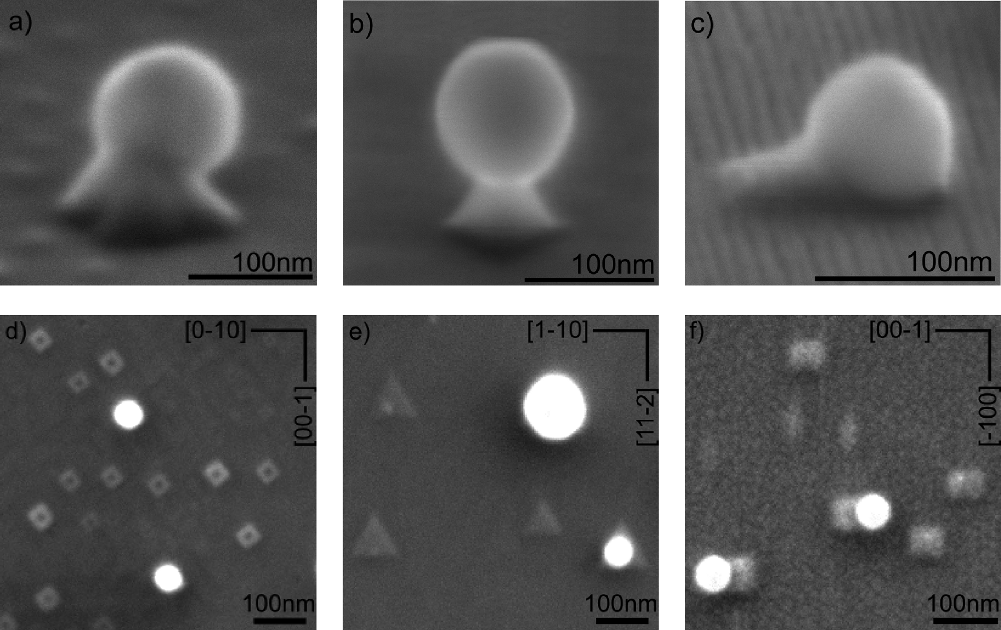
\includegraphics{nanogold_sem}
    \caption{\label{fig:nanogold_sem}SEM images showing the gold nanostructures formed
        on MgAl2O4 substrates. The three upper images show spheres
        supported by a necking region attached to a geometrically shaped
        base for the (a) [100]-, (b) [111]-, and (c) [110]-oriented substrates.
        Each of these images was taken at a 70°\degree tilt. The aura seen around
        nanostructures is an artifact of imaging. The three lower images
        show the top-down view of both standalone base structures and
        supported spheres for the (d) [100]-, (e) [111]-, and (f) [110]-
        oriented substrates. The in-plane Miller indices of the substrate are
        denoted on each of these images. For all cases, the samples were
        coated with a thin layer of platinum to improve imaging. Imaging
        without platinum shows the same structures but is of poor quality
        due to substrate charging effects.}
\end{figure}
While there are two basic types of nanostructures formed
on each substrate orientation, these structures are found in
various stages of development. For the most part, the bases
are well-developed and show little size variation. The
spherical structures, however, vary dramatically both in their
size and position relative to the base structures. Figure 2
shows a series of top-down SEM images for the case of the
(111) MgAl2O4 substrate showing an evolution of the
nanostructures from a standalone triangular base to bases
supporting spheres of increasing size. Notable is the fact that
the nanostructure, shown in Figure 2b, manifests itself as a
small sphere which is offset from the center of the base while for the larger spheres, this asymmetry disappears. Such
asymmetries are observed for all three substrate orientations,
but only those nanostructures formed on the (111) substrate
consistently show a centrally placed sphere for the large
sphere sizes. Also noteworthy is a systematic effect whereby
the size of the triangular base structure increases for sphere
diameters greater than 80 nm (see Figure 2e and f).
\begin{figure}
    \centering
    \missingfigure{SEM Progression of figure}
    \caption{\label{fig:nanogold_progression}SEM images showing the top-down view of gold
        nanostructures formed on the (111) surface of MgAl2O4 substrates.
        The sequence of images is chosen to show progressively larger
        spheres atop the base structures. Note that only the smallest sphere,
        shown in (b), is offset from the center of the triangular base and
        that the base size is slightly larger when supporting larger spheres,
        as is the case for (e) and (f). The size of each image is 130$\times$30
        nm\textsuperscript{2}.}
\end{figure}
The base structures formed on each substrate orientation
are a clear consequence of the epitaxial relationship formed
between gold and the latticed-matched MgAl2O4 substrate.
This is apparent from the fact that the geometries of the base
structures mimic the underlying symmetry of the substrates.
It is also likely that the base sizes are a consequence of the
substrate-imposed strains. Arguments based on epitaxy,
however, cannot explain the self-assembly of the gold spheres
atop the base structures and the associated necking behavior
which facilitates their connection to the base. It is our
hypothesis that the necking behaviour results from an attempt
to minimize the surface energy of the structure. Thus, the
overall shape of these nanostructures is governed by an
interplay between the constraints imposed by epitaxy and a
requirement that the surface free energy be minimized. This
situation has much in common with formation of soap
bubbles affixed to a wire frame.38 This statement is based
on the facts that the frame imposes a constraint analogous
to that imposed by lattice mismatch and that the shape of
the soap bubble is, to a large degree, determined by the
surface free energy. This analogy provided the impetus for
applying the well-developed models associated with soap
bubble formation to the nanostructures described here. Such
modelling has also been successfully used to predict the
equilibrium shape of biological lipid bilayers (blood cells)
when exposed to abnormal pressure, temperature, magnetic,
and chemical environments.39-44
\section{Implications for Symmetry and Energy at Epitaxial Surfaces}